\documentclass[11pt]{report}
\usepackage[margin=1in]{geometry}
\usepackage{titlesec}
\usepackage{graphicx}
\usepackage{parskip}
\usepackage{glossaries}
\usepackage{datetime}

\titleformat{\chapter}{\Large\bfseries}{}{0pt}{\huge}
\titlespacing\chapter{0pt}{*1}{*1}
\titlespacing\section{0pt}{*0}{-\parskip}
\titlespacing\subsection{0pt}{*0}{-\parskip}
\titlespacing\paragraph{0pt}{*0}{*3}

\newcommand*{\TitleFont}{
      \usefont{\encodingdefault}{\rmdefault}{b}{n}
      \fontsize{24}{36}
      \selectfont
}
\newcommand{\thickline}{\rule{\textwidth}{1.6pt}}
\newcommand{\thinline}{\rule{\textwidth}{0.4pt}}
\newcommand{\novspace}{\vspace*{-\baselineskip}\vspace*{4pt}}
\renewcommand{\dateseparator}{-}
\let\oldtitle\title
\renewcommand{\title}[1]{\oldtitle{\thickline \\ \novspace \thinline \\ \TitleFont {#1} \thinline \\ \novspace \thickline}}
\newcommand{\tableoffiguresandtables}{\listoffigures\begingroup\let\clearpage\relax\listoftables\endgroup}

\author{
	Evan Milton \\
	Computer and Electronics Engineering \\
	University of Nebraska at Lincoln - Omaha Campus \\
	Electronics Engineering
		\and
	Josh DeWitt \\
	Computer and Electronics Engineering \\
	University of Nebraska at Lincoln - Omaha Campus \\
	Computer Engineering and Mathematics, minor in Computer Science
		\and
	Chad Staley \\
	Computer and Electronics Engineering \\
	University of Nebraska at Lincoln - Omaha Campus \\
	Electronics Engineering
		\and
	James Gehringer \\
	Computer and Electronics Engineering \\
	University of Nebraska at Lincoln - Omaha Campus \\
	Computer Engineering, minor in Computer Science
}
\date{\yyyymmdddate\today}

\newacronym{2d}{2-D}{Two-Dimensional}
\newacronym{3d}{3-D}{Three-Dimensional}
\newacronym{aon}{AON}{Activity On Node}
\newacronym{arm}{ARM}{Advanced RISC Machines}
\newacronym{bom}{BOM}{Bill of Materials}
\newacronym{cad}{CAD}{Computer-Aided Design}
\newacronym{ceen}{CEEN}{Computer and Electronics Engineering}
\newacronym{cnc}{CNC}{Computer Numerical Control}
\newacronym{cpu}{CPU}{Central Processing Unit}
\newacronym{dmm}{DMM}{Digital Multi-Meter}
\newacronym{drc}{DRC}{Design Rules Check}
\newacronym{dvi}{DVI}{Digital Visual Interface}
\newacronym{eco}{ECO}{Engineering Change Order}
\newacronym{ecr}{ECR}{Engineering Change Request}
\newacronym{gpio}{GPIO}{General Purpose Input/Output}
\newacronym{led}{LED}{Light Emitting Diode}
\newacronym{lrc}{LRC}{Linear Responsibility Chart}
\newacronym{pcb}{PCB}{Printed Circuit Board}
\newacronym{pi}{Pi}{Raspberry Pi}
\newacronym{pcsc}{PCSC}{Project Common Success Criteria}
\newacronym{pssc}{PSSC}{Project Specific Success Criteria}
\newacronym{tcpip}{TCP/IP}{Transmission Control Protocol/Internet Protocol}
\newacronym{ti}{TI}{Texas Instruments}
\newacronym{wbs}{WBS}{Work Breakdown Structure}
\newacronym{xp}{XP}{Extreme Programming}

\date{2013-12-12}
\titleandsubtitle{CNC Interface \\ Team 3 - Project Proposal}{A planning document for a Senior Thesis Project submitted to the faculty of \\ Computer and Electronics Engineering \\ University of Nebraska-Lincoln \\ College of Engineering \\ Peter Kiewit Institute}

\begin{document}
\maketitle
\tableofcontents
\tableoffiguresandtables

\chapter{Project Definition}
The purpose of this Senior Thesis Project is to create a \gls{cnc} interface, capable of receiving standardized G-code through \gls{tcpip}, processing the G-code, and driving motors and \gls{gpio} according to the G-code. 

\section{Project Need}
The modern \gls{cnc} interface is limited to utilization of a full computer system, in combination with a motor driver platform to for complete functional control.
This setup can cost upwards of \$500, depending on the quality and system specifications.
This system will encapsulate these hardware and software requirements completely for less than \$100, bringing the \gls{cnc} interface to a price point comparable with that of the modern printer. 

\section{Existing Solutions}
\gls{cnc} system requirements currently rely upon complex computer-driver interfaces to control the machine.
The system requires a complete software package operating from a PC to manipulate an entirely separate set of motor drives running the machine.
While this may be practical for commercial and industrial applications, many of the features provided by this system will not be utilized by the average consumer.

\section{Existing Solutions Improvement}
This project will encapsulate these hardware and software requirements completely within a system costing less than \$100.
In combination of the basic functions provided by the PC with the root functionality of the motor driver unit, the system as a whole can be greatly simplified.
The addition of a Web-Interface will allow for users to operate the \gls{cnc} remotely.
This will bring system functionality to a level on par with the modern printer.

\section{Project Scope}
The \gls{cnc} interface will be configurable to operate on different mechanical systems. 
The scope includes the software for the G-code interpretation, its upload interface, the master controller, the motor controller and the motor driver board.
The G-code interpretation software will have a G-code file as an input and output motor driver commands from the master controller to the motor controller.
The motor controller will send out the driver signals to the motor driver board. 
The motor driver board will take the command outputs from the motor controller and then drive the motors. 
There will be 16 \gls{gpio} pins, an emergency stop switch, and home switches for the motors. 

\section{Marketing Requirements}
The system will meet the following criteria:
\begin{enumerate} \parskip2pt
	\item be accurate in its motor control.
	\item be able to quickly accelerate the motors.
	\item be able to send command files through a web interface.
	\item be able to drive multiple motors.
	\item be able to handle general purpose input and output.
	\item be able to be stopped in an emergency.
	\item be able to shutdown if the system gets too hot. 
	\item be able to operate at a range of input voltages.
\end{enumerate}

\section{Objective Tree}
~\ref{fig:o-tree} outlines the requirements for having a functioning \gls{cnc} interface for this Senior Thesis Project.
Safety is the most important objective in this project since the \gls{cnc} interface will control moving components, although these moving components are outside the scope of this report.
Next most important is the \gls{cnc} functionality, otherwise the interface would not be able to control any \gls{cnc}
Speed and accuracy is rated next most important to ensure the movements coordinated by the interface are as closed to the desired as possible.
The \gls{cnc} control is required to allow G-Code to be uploaded to the system and allow system monitoring.
A variable power input is desired so that users may purchase a power supply that fits their motors' needs, ensuring that a properly priced power supply is bought for the system.

\begin{figure}[H]
\centering
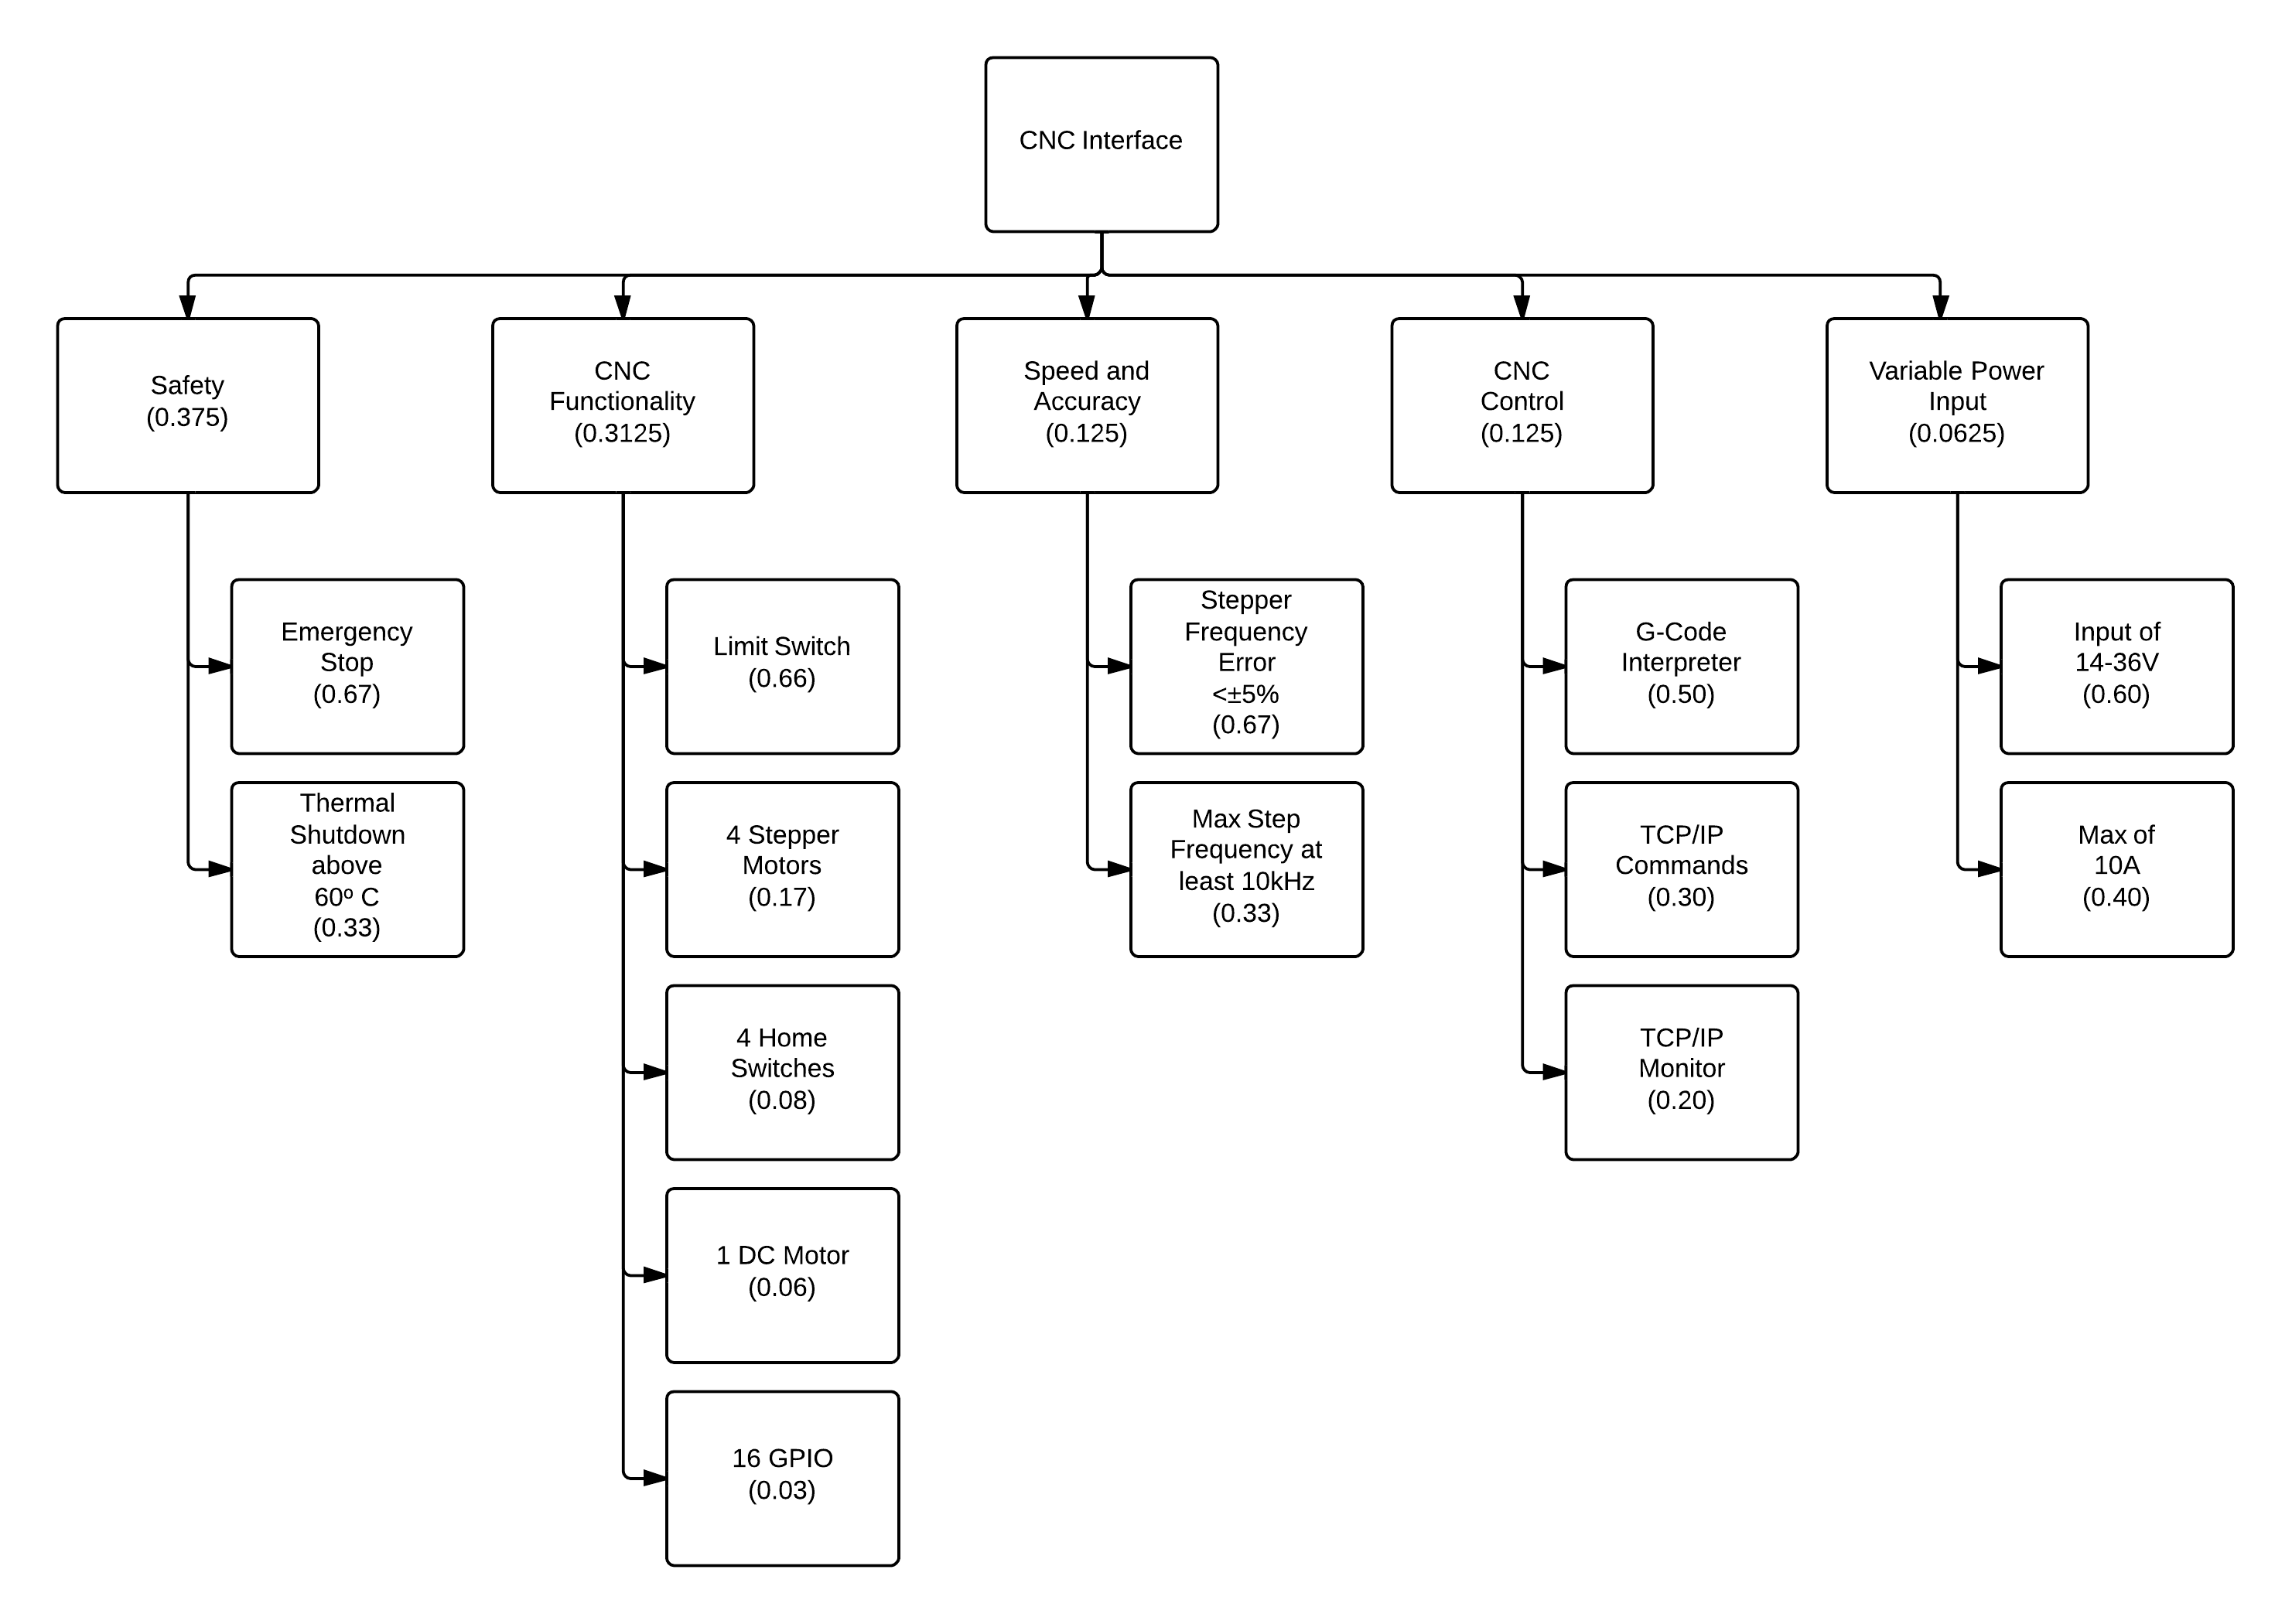
\includegraphics[width=1.0\textwidth]{otree.png}
\caption{Objective Tree}
\label{fig:o-tree}
\end{figure} 

\section{CEEN Appropriateness}
The design and execution of the CNC Interface will meet at least 7 of the 11 ABET accreditation criteria.
The design and construction will require the rigorous application of mathematics, science, and engineering for the software, hardware, mechanical, and system control. (ABET 3a).
Notably, the kinematics of the robot will require intense mathematical computations to ensure accuracy.
Experiments must be designed and conducted to ensure proper operation of components and the final result (ABET 3b).
The end result of the project will meet the needs outlined in the Background Summary (ABET 3c).
The level of success of the project will depend on how well the the team is able to cooperate and strive to achieve common goals (ABET 3d).
This project will present many engineering problems that will have to be solved (ABET 3e).
Not only must the group work towards common goals, but they must also communicate effectively (ABET 3g).
Similarly to ABET 3a, the entire project will involve the use of engineering skills that have been learned in previous coursework (ABET 3k).

The Senior Thesis Project also serves as a culmination of the CEEN curriculum. Concepts and skills learned in previous courses must be applied in the design, construction, and documentation of the project.
Courses that will be built upon in the design of the CNC interface are:
\begin{enumerate} \parskip2pt
	\item Microprocessor Applications
	\item Electrical \& Electronic Circuits
	\item Communication Systems
	\item Signals \& Linear Systems
	\item Digital Design \& Interface
	\item Microprocessor System Design
	\item Embedded Microcontroller Design
\end{enumerate}

\chapter{Engineering Requirements Specification}

\section{Five \gls{pcsc}}
\begin{enumerate}
	\item Create a complete \gls{bom} and order/sample all parts needed for the design.
	\item Develop complete, accurate, readable schematic of the design, complete with interface loading analysis and interface timing analysis. 
	\item Complete a layout and etch a \gls{pcb}.
	\item Populate and debug the design on a custom \gls{pcb}.
	\item Professionally package the finished product and demonstrate its functionality.
\end{enumerate}

\section{Five \gls{pssc}}\
\begin{enumerate}
	\item The system will drive at least 4 stepper motors, 1 DC motor, and 16 \gls{gpio}.
The system will receive inputs from at least 1 motor limit/emergency stop switch and 4 stepper motor home inputs.
	\item The system will Receive G-code through \gls{tcpip}.
The system’s software will be developed using IEEE Std 830-1998 Recommended Practice for Software Requirements Specifications.
	\item The maximum step frequency will be at least 10kHz.
The target step frequency will be within 5\% of the desired frequency.
	\item The system power supply will accept between 14V and 36V and draw a maximum of 10A.
	\item The system will enter thermal shutdown above CPU temperatures of $60^{\circ}C$ and the motors will cease to operate.
\end{enumerate}

\section{Requirements Validation}
Table ~\ref{table:Val} shows the relationship between the five \gls{pssc} and the marketing requirements.
For a marketing requirement to be validated, the respective engineering requirements must be verified.

\begin{table}[ht]
	\caption{Engineering Requirement vs. Marketing Requirements}
	\label{table:Val}
	\centering
	\begin{tabular}{|r |c |c |c |c |c|} 
		\hline\hline
		&1&2&3&4&5\\
		\hline
		\textbf{Accurate} &  & & X & X & \\
		\hline
		\textbf{Quick} &  & & X & X & \\
		\hline
		\textbf{Web Interface} & & X & & & \\
		\hline
		\textbf{Drive Motors} & X & & X & X & \\
		\hline
		\textbf{Handle \gls{gpio}} & X & & & X & \\
		\hline
		\textbf{Emergency Stop} & X & & & X & \\
		\hline
		\textbf{Thermal Shutdown } & X & & & X & X \\
		\hline
		\textbf{Supply Range} & & & & X &   \\

	\hline 
	\end{tabular}
\end{table}
\chapter{Design Alternatives Generation}
A prior goal of this project was to deliver a Delta style \gls{3d} printer.
While this would have delivered a \gls{3d} printer, calculating the movement of the work head and applying it to the acceleration of the motors proved to be a large undertaking that would have been difficult to accomplish in the time allotted.
The current focus of a \gls{cnc} driver will instead be a starting point for any \gls{3d} design including Delta and Cartesian \gls{3d} printers.

Other design alternatives that were considered were the choices for the central processor and motor drivers.
Ultimately, the \gls{pi} was chosen as the processor but another consideration was the BeagleBone Black.
While the BeagleBone Black boasts faster processing speed and more outputs, the \gls{pi} was chosen for its lower cost and available support.
The motor controller chosen was the \gls{ti} DRV8825 over the alternative Allegro A4988. The \gls{ti} DRV8825 has greater step resolution and accepts a larger range of input voltage.

Due to the possibility of timing and overhead issues while timing the movement of 4 stepper motors it was decided that a microcontroller would be used to handle the motor control.
The microcontroller that will be used for this project remains to be determined, but considerations include the TI MSP430 and various Atmel microcontrollers.

\section{Web Interface}
There are four approaches to the interface, using PHP, Javascript, HTML5 or building a stand alone application.
They will be evaluated based on their ability to create a GUI, the current team knowledge and the community knowledge base available. 

PHP gives a fine selection of tools to create a GUI.
The team also has a solid foundation in PHP development.
PHP also has a large community for development and support.

Javascript is well known for its GUI capabilities, offering many different libraries and functions to create dynamic interfaces. 
The team is also knowledgeable on development through Javascript.
The Javascript community is very active and offers a lot of support.

HTML5 has the ability to create dynamic interfaces.
The team does have background in HTML5.
The HTML5 documentation and support is not as strong as PHP or Javascript's communities are.

A stand alone application will give complete control over a GUI.
The team does not have much knowledge of how to build a stand alone application, compared to writing in PHP, Javascript, or HTML5.
There will not be much support when building a stand alone application.

\section{Master Controller}
\paragraph{Rasberry Pi}
The \gls{pi} is a single board computer developed by the Rasberry Pi Foundation (RPF) to promote computer science education in schools worldwide.
It is based off of the Broadcom BCM2835 System on a Chip (SOC) featuring a 700 MHz ARM processor, VideoCore IV GPU, and 512 MB of Random Access Memory (RAM).
This enables the Pi to maintain a complete Linux Operating System (OS), at a price point just under 35 US Dollars (USD).
Of major benifit to the Pi is the community that has emerged to support its development post-launch.

\paragraph{BeagleBoard}
The BeagleBoard (BB) is a single board computer developed by Texas Instruments (TI) for the Digi-Key and Newark consumer markets.
It is based off of the OMAP3530 SOC featuring a 600 MHz ARM processor, TMS320C64+ DSP, and 256 MB of RAM.
This enables the BeagleBoard to operate a variety of Linux OS’s, for a cost of 45 USD.
Of major benifit to the BB is its well documented and supported development cycle, as provided by TI.

\paragraph{Arduino Mega}
The Arduino platform is a grouping of microcontroller implementations that utilize the AVR \& ARM chip archtectures, in combination with a custom compiler.
The most powerful device in this series is the Arduino Mega, with a 16 MHz clock speed has 128 KB of meory, and 54 digital GPIO pins.
While not capable of running an entire OS, this microcontroller offers direct register access and is ethernet capable.
The Arduino community is also one of the most active open source hardware communities alive on the web today.


\section{Motor Driver Controller Microcontroller}
There are four microcontrollers that were evaluated for use in the Motor Driver Controller board, the MSP430, the ATMega324P, the AT90USB1287, and the ARM Stellaris.
These microcontrollers were evaluated based on the number of timers they had, their interrupt capabilities, their SPI capabilities and the number of GPIO pins.

The MSP430 has 5 timers, which is more than what the project will need.
It does have interrupt capabilities.
The MSP430 does handle SPI communication. 
There is up to 90 GPIO pins.

The ATMega324P has 3 timers.
There are interrupt capabilities with this microcontroller.
A master/slave SPI serial interface is available.
There are 32 GPIO pins.   

The AT90USB1287 has 4 timers, which is what the project needs.
There are interrupt capabilities with this microcontroller.
There are two SPI ports available. 
There are 48 GPIO pins.

The ARM Stellaris has 3 timers.
There are interrupt capabilities with this microcontroller.
It has one SPI port available.
There are up to 36 GPIO pins.

\section{Motor Drivers}
\paragraph{DRV8825}
The DRV8825 is a microstepping bipolar stepper motor driver manufactured by TI.
It features adjustable current limiting, overcurrent and overtemperature protection, and six microstep resolutions (down to 1/32-step).
It operates from 8.2 45 V and can deliver up to approximately 1.5 A per phase without a heat sink or forced air flow (rated for up to 2.2 A per coil with suffcient additional cooling).

\paragraph{A4988}
In the same vein as the DRV8825, the A4988 is a microstepping bipolar stepper motor driver manufactured by Allegro.
The driver features adjustable current limiting, overcurrent and overtemperature protection, and five different microstep resolutions (down to 1/16-step).
It oper- ates from 8 35 V and can deliver up to approximately 1 A per phase without a heat sink or forced air flow (it is rated for 2 A per coil with suffcient additional cooling).

\paragraph{TB6560}
The TB6560 is a Pulse Width Modulation (PWM) chopper-type stepping motor driver IC designed for sinusoidal-input microstep control of bipolar stepping motors.
The TB6560 can be used in applications that require 2-phase, 1-2-phase, 2W1-2-phase and 4W1-2-phase excitation modes.
The TB6560 is capable of low-vibration, high-performance forward and reverse driving of a two-phase bipolar stepping motor using only a clock signal.
\chapter{Design Alternatives Evaluation}
Evaluations of design alternatives are shown Tables ~\ref{table:TCPIP} through ~\ref{table:MCEval}.


\section{TCP/IP Interface}
Since sensitive data will not be shared with the device, security is not required, though it is preferred. 
Since plaintext or SSL sockets and SFTP are more difficult to use than the other options, they should not be used since the final product should not require special training. 
HTTPS will be used for its security advantages over HTTP, and ease of use over other methods. 

\begin{table}[h]
\caption{Web Interface Evaluation}
	\label{table:TCPIP}
	\centering
\begin{tabular}{|r|c|c|c|c|c|c|}
\hline
Item              	& Weight & HTTPS  & HTTP       & SFTP        & SSL Socket	& Plaintext\\ \hline
Security       	& 1      & -      & -1         & 0           & 0          	& -1   \\ \hline
Implementation	& 2      & -      & 1          & 0           & -1     		& 1   \\ \hline
Ease of Use       	& 3      & -      & 0          & -1          & -1         	& -1 \\ \hline
Score         	&        & -      & 1          & -3          & -5         	& -2   \\ \hline
Alternative     	&        & Y      & Y          & N           & N       	& N   \\ \hline
\end{tabular}
\end{table}

\section{Master Controller}
The \gls{pi} was selected from the following alternitives for its superior hardware, and application notes.
\begin{table}[H]
\caption{Master Controller Evaluation}
	\label{table:MaCEval}
	\centering
\begin{tabular}{|r|c|c|c|c|}
\hline
Item              & Weight & RasPi & Beagle &Arduino \\ \hline
Speed             & 1      & -     & 0                                                     & -1                                                     \\ \hline
Versatility       & 3      & -     & 0                                                     & 0                                                      \\ \hline
GPIO              & 2      & -     & 1                                                     & 1                                                      \\ \hline
Application Notes & 4      & -     & -1                                                    & 0                                                      \\ \hline
Score             &        & -     & -2                                                    & 1                                                      \\ \hline
Alternative       &        & Y     & N                                                    & Y                                                    \\ \hline
\end{tabular}
\end{table}

\section{Motor Driver Controller Microcontroller}
Of the following alternatives, the MSP430 was selected for its low cost, adequate timer count, and interrupt capabilities.
\begin{table}[H]
\caption{Motor Controller Evaluation}
	\label{table:uCEval}
	\centering
\begin{tabular}{|r|c|c|c|c|c|}
\hline
Item              	& Weight & MSP430 & ATMega324P & AT90USB1287 & ARM Stellaris \\ \hline
GPIO          	& 1      & -      & 1          & 1           & 1             \\ \hline
SPI         		& 2      & -      & 0          & 0           & 0             \\ \hline
Interrupt			& 3      & -      & 0          & 0           & 0             \\ \hline
Timers        	& 4      & -      & -1         & -1          & 1             \\ \hline
Score         	&        & -      & -3         & -3          & 5             \\ \hline
Alternative     	&        & Y      & N          & N           & Y           \\ \hline
\end{tabular}
\end{table}

\section{Motor Drivers}
Of the following alternatives, the DRV8825 was selected for its comparable power capabilities, and superior documentation.
\begin{table}[H]
\caption{Motor Drivers Evaluation}
	\label{table:MCEval}
	\centering
\begin{tabular}{|r|c|c|c|c|}
\hline
Item                   & Weight & DRV8825 & A4988 & TB6560 \\ \hline
Microstepping 	 	& 1      & -       & -1    & -1     \\ \hline
Price                  & 2      & -       & 1     & 1      \\ \hline
Failsafe               & 3      & -       & 1     & -1     \\ \hline                         
Power Output           & 4      & -       & -1    & -1     \\ \hline
Score                  &        & -       & 0     & -6     \\ \hline
Alternative            &        & Y       & Y     & N      \\ \hline
\end{tabular}
\end{table}



\chapter{Functional Breakdown of Selected Design}
The main microprocessor, an \gls{arm} 11 on the \gls{pi}, will be responsible for controlling the three stepper motors for the CNC.
This objective will be achieved by creating a G-code interpreter written in C.
The microprocessor will be responsible for scheduling movements to make smooth transitions to the destination, as interpreted from the G-code.

The system will be a network device, connected through WiFi or Ethernet.
The microprocessor will obtain G-code commands through local storage or by accepting G-code files over TCP/IP.
The G-code received over TCP/IP and will be stored locally for reuse in the future.
Execution of G-code sequences will be started through a TCP/IP interface.
All network interfaces will be password protected and use encryption algorithms to ensure that all commands executed are from authorized users. 

A secondary microprocessor may be required to precisely control stepper motors and the \gls{gpio}.
This secondary microprocessor will perform any required communication with the network-connected main microprocessor through a serial interface. 

\section{Level Zero Breakdown}
Figure ~\ref{fig:architecture} shows the overall architecture of the Senior Thesis Project, which is fully specified by Table ~\ref{table:zerolevel}.

\begin{figure}[h]
	\centering
	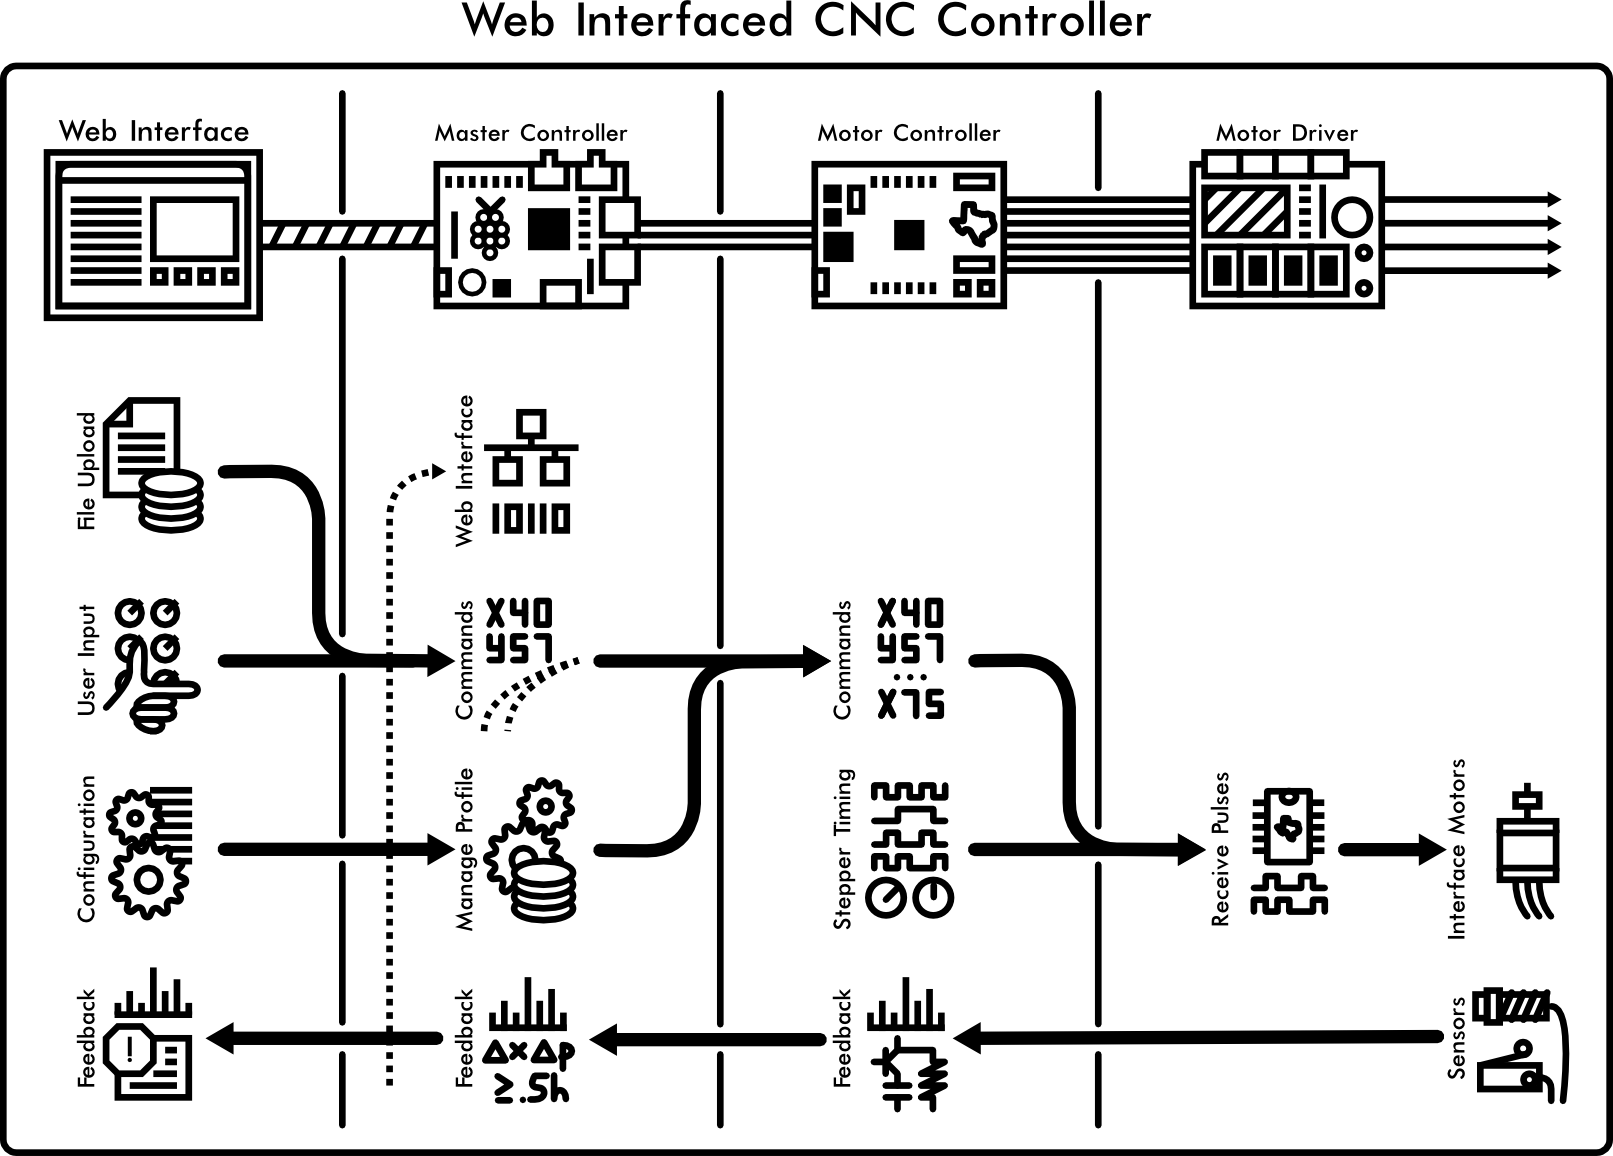
\includegraphics[width=1\textwidth]{architecture.png}
	\caption{System Architecture}
	\label{fig:architecture}
\end{figure}

\begin{table}[h] 
	\caption{Zero Level Module Definition}
	\label{table:zerolevel}
	\centering 
	\begin{tabular}{|r p{10cm}|} 
		\hline\hline
		Module		& Web Interfaced CNC Controller \\ 
		Inputs		& User Commands \& Data files 	\\ 
		Outputs		& Motor Commands \& Feedback	\\ 
		Functionality	& This device will enable users to control CNC systems via a web-based interface 	\\ 
		\hline
		\end{tabular} 
\end{table}

\section{Level One Breakdown}
Table ~\ref{table:firstlevel} specifies the definitions for the Level One components of the Senior Thesis Project. 
\begin{table}[H] 
	\caption{First Level Module Definition}
	\label{table:firstlevel}
	\centering 
	\begin{tabular}{|r p{10cm}|} 
		\hline\hline 
		Module		& Web Interface \\ 
		Inputs		& User Commands \& Data files, Master Control Feedback	\\ 
		Outputs		& Master Control Commands \& User Feedback \\ 
		Functionality	& This device will enable users to control CNC systems via a web-based interface by communicating with the Master Controller.\\ 
		\hline\hline 
		Module		& Master Control Board \\ 
		Inputs		& Master Control Commands \& Motor Controller Feedback	\\ 
		Outputs		& Motor Control Commands \& Web Interface Feedback \\ 
		Functionality	& This device will receive commands over the Internet, and interface them with the Motor Control Board. \\
		\hline\hline 
		Module		& Motor Control Board \\ 
		Inputs		& Motor Control Commands \& Sensor Feedback	\\ 
		Outputs		& Motor Driver Commands \& Master Controller Feedback \\ 
		Functionality	& This device will be responsible for realtime management of motor timing, and interfacing with the Motor Driver. It will also convert sensor feedback for the Master Control Board.\\
		\hline\hline 
		Module		& Motor Driver Board \\ 
		Inputs		& Motor Driver Commands \\ 
		Outputs		& Electronic control of Stepper Motors \\ 
		Functionality	& This device will manage the power and step-modes nessescary to manipulate the stepper motors based on the Motor Controller's commands. \\
		\hline\hline 
		Module		& Power Supply Unit \\ 
		Inputs		& Mains Voltage	\\ 
		Outputs		& Various Voltage Levels \\ 
		Functionality	& This device will manage power for the CNC Controller portion of the build. \\
		\hline
		\end{tabular} 
\end{table}

\section{Level Two Breakdown}
Tables ~\ref{table:secondlevelweb} through ~\ref{table:secondleveldriver} specify the definitions for the Level Two components of the Senior Thesis Project.
\begin{table}[H] 
	\caption{Second Level Module Definition - Web Interface}
	\label{table:secondlevelweb}
	\centering 
	\begin{tabular}{|r p{10cm}|} 
		\hline\hline 
		Module		& File Upload \\ 
		Inputs		& G-Code Files, Gerber Files, External Commands	\\ 
		Outputs		& Master Control Commands \\ 
		Functionality	& This unit will control conversion of User Data to Master Controller Commands.\\ 
		\hline\hline 
		Module		& Command Execution \\ 
		Inputs		& User Commands	\\ 
		Outputs		& Master Control Commands \\ 
		Functionality	& This unit will accept user commands (Left, Right, Stop) and convert them to the Master Controller Format.\\
		\hline\hline 
		Module		& Configure Machine \\ 
		Inputs		& User Input \\ 
		Outputs		& Master Control Commands \\ 
		Functionality	& This unit will be responsible for converting the User Machine Configuration information into Master Controller Commands.\\
		\hline\hline 
		Module		& Feedback Reception \\ 
		Inputs		& Master Controller Feedback \\ 
		Outputs		& User Feedback \\ 
		Functionality	& This unit will interpret feedback from the Master Controller, and present it to the end User. \\
		\hline
		\end{tabular} 
\end{table}

\begin{table}[H] 
	\caption{Second Level Module Definition - Master Control Board}
	\label{table:secondlevelmaster}
	\centering 
	\begin{tabular}{|r p{10cm}|} 
		\hline\hline 
		Module		& Web Interface \\ 
		Inputs		& Internet Data	\\ 
		Outputs		& Master Control Commands \\ 
		Functionality	& This unit will be responsible for interpreting data in the TCP/IP format for use as Master Control Commands.\\ 
		\hline\hline 
		Module		& Machine Profile Maintainence \\ 
		Inputs		& Master Control Commands (User Input)\\ 
		Outputs		& Local configuration settings \\ 
		Functionality	& This unit will store information about the CNC configuation locally for use in processing operations.\\
		\hline\hline  
		Module		& Command Processing \\ 
		Inputs		& Master Control Commands (User Commands \& G-Code etc.) \\ 
		Outputs		& Motor Control Commands \\ 
		Functionality	& This unit will calculate the desired course of action based off of the Machine Profile, and pass it to the Motor Controller.\\
		\hline\hline 
		Module		& Feedback Management \\ 
		Inputs		& Motor Controller Feedback \\ 
		Outputs		& Web Interface Feedback \\ 
		Functionality	& This unit will interpret feedback from the Motor Controller, and present it to the Web Interface. \\
		\hline
		\end{tabular} 
\end{table}

\begin{table}[H] 
	\caption{Second Level Module Definition - Motor Control Board}
	\label{table:secondlevelmotor}
	\centering 
	\begin{tabular}{|r p{10cm}|} 
		\hline\hline 
		Module		& Command Reception \\ 
		Inputs		& Motor Control Commands	\\ 
		Outputs		& Motor Driver Commands \\ 
		Functionality	& This unit will be responsible for processing position commands from the Master Controller.\\ 
		\hline\hline 
		Module		& Stepper Management \\ 
		Inputs		& Motor Control Commands \\ 
		Outputs		& Motor Driver Commands \\ 
		Functionality	& This unit will process the Motor Control Commands, and calculate the Step Frequency for real-time operation.\\
		\hline\hline  
		Module		& Feedback Management \\ 
		Inputs		& Sensor Feedback \\ 
		Outputs		& Master Controller Feedback \\ 
		Functionality	& This unit will interpret feedback from the Feedback Sensors, and present it to the Master Controller. \\
		\hline
		\end{tabular} 
\end{table}

\begin{table}[H] 
	\caption{Second Level Module Definition - Motor Driver Board}
	\label{table:secondleveldriver}
	\centering 
	\begin{tabular}{|r p{10cm}|} 
		\hline\hline 
		Module		& Command Reception \\ 
		Inputs		& Motor Driver Commands	\\ 
		Outputs		& Interface with Motor \\ 
		Functionality	& This unit will be responsible for allowing pulses from the Motor Control board to manipulate the Stepper Motors.\\
		\hline
		\end{tabular} 
\end{table}
\chapter{Project Plan}
\section{Risk Management Procedure}
Certain risks will be faced throughout the project, though proper avoidance and mitigation plans will allow project objectives to be completed on time.
Risks will be obsessed using AHP and pairwise comparisons.
If possible, quantitative measurements, in terms of financial or class grade loss if the risk is realized, will allow comparison to determine which risks will be focused on to ensure that they are not realized.

\subsection{Risk Identification}
From previous experience, the major risks that will occur in the project will likely be related to increasing scope, unfeasible designs, insufficient resources, delayed shipments, and lack of motivation.

\subsection{Risk Avoidance}
\begin{itemize} \parskip2pt
	\item To avoid increasing scope late in the project, there will be a change moratorium to the project's scope at the end of the Senior Thesis proposal class.
Any additional substantial features must be put on hold until the end of the semester if time permits; all other requirements must first be completed.
	\item To avoid issues from a design becoming unfeasible, viable alternative designs will be created in the planning phase.
	\item To avoid running short of resources, proper resource management and thorough time and money planning will ensure that all resource expenditure is within budget.
	\item To avoid being affected by delayed shipments, parts will be ordered as soon as they are confirmed to be required.
	\item To avoid slipping motivation, the team will be kept in contact to create an atmosphere of team cooperation and ensure that all team members feel useful in the project.
\end{itemize}	

\subsection{Risk Mitigation}
\begin{itemize}
	\item In the case of required increased project scope, the team will collaborate and decide the new priority of tasks using AHP. 
The tasks will be worked in the order decided, and the team will understand which items may not be completed in time.
	\item In case a design becomes unfeasible, one of the alternate designs created in the planning phase will be pursued.
	\item In case of insufficient financial resources, the investors will be contacted, or more investors will be located to sponsor the project.
	\item If shipments are delayed, alternative distributors will be researched and ordered from to obtain the part in time.
	\item If there is a lack of motivation on the team, team outings will be planned that do not involve the project, but will allow team bonding and any personal issues to be discussed.
\end{itemize}

\section{Change Management Procedure}
Any major changes to the design will be decided with a meeting that includes all the effected developers.
Once a change has been decided on, the Resource Manager will complete the paperwork for an \gls{ecr}.
This will be submitted to Professor Detolff for review.
If the change is approved, an \gls{eco} will be used to direct the change.

\section{Work Breakdown Structure}
\begin{longtable}{|c|m{4cm}|m{4cm}|>{\centering}m{1.6cm}|m{3.5cm}|}
	\caption{Work Breakdown Structure}
	\label{table:primary} \\
	\hline \textbf{ID} & \textbf{Activity} & \textbf{Deliverable} & \textbf{Duration (Days)} & \textbf{Resources} \\ \hline
	\endfirsthead
	\multicolumn{5}{c}{\tablename\ \thetable\ -- \textit{Continued from previous page}} \\ \hline
	\textbf{ID} & \textbf{Activity} & \textbf{Deliverable} & \textbf{Duration (Days)} & \textbf{Resources} \\ \hline
	\endhead 
	\multicolumn{5}{r}{\textit{Continued on next page}} \\
	\endfoot \hline
	\endlastfoot

	\hline 1.1 & \multicolumn{4}{c|}{Electrical Components} \\ \hline
	1.1.1 & Construct test board & LED testing breakout & 7 & Components\newline Perfboard \\ \hline
	1.1.2 & \multicolumn{4}{l|}{Motor Driver Prototype} \\ \hline
	1.1.2.1 & Design motor driver PCB & Shield PCB & 30 & Eagle\newline \gls{cnc}\newline Components \\ \hline
	1.1.2.2 & Order motor drivers & Motor drivers & 1 & Computer \\ \hline
	1.1.2.3 & Construct sensor circuitry & Sensor circuitry & 14 & Eagle\newline \gls{cnc}\newline Components \\ \hline
	1.1.2.4 & Construct power supply & Power & 7 & Eagle\newline \gls{cnc}\newline Components \\ \hline
	1.1.3 & Send final motor driver PCB design to boardhouse & Final motor driver & 14 & Eagle\newline \gls{cnc}\newline Components \\ \hline
	1.1.4 & Construct work head controller & Work head controller & 17 & Eagle\newline \gls{cnc}\newline Components \\ \hline
	\hline 1.2 & \multicolumn{4}{c|}{Control Software} \\ \hline
	1.2.1 & \multicolumn{4}{l|}{LED Control Software} \\ \hline
	1.2.1.1 & Research \gls{pi} \gls{gpio} & Pi \gls{gpio} knowledge & 4 & Computer \\ \hline
	1.2.1.2 & Program for \gls{pi} \gls{gpio} & LED controller & 3 & Computer \\ \hline
	1.2.2 & \multicolumn{4}{l|}{Motor Control Software} \\ \hline
	1.2.2.1 & \gls{gpio} Timing research & \gls{gpio} timing understanding & 5 & Computer \\ \hline
	1.2.2.2 & Program motor controller & Motor controller software & 10 & Computer \\ \hline
	1.2.3 & \multicolumn{4}{l|}{Kinematics Control Software} \\ \hline
	1.2.3.1 & Research kinematics requirements & Kinematics equations & 5 & Computer\newline Calculator \\ \hline
	1.2.3.2 & Program kinematics equations & Kinematics software & 10 & Computer \\ \hline
	1.2.4 & \multicolumn{4}{l|}{G-code Interpreter} \\ \hline
	1.2.4.1 & G-code research & G-code understanding & 7 & Computer \\ \hline
	1.2.4.2 & Program G-code interpreter & G-code Software & 14 & Computer \\ \hline
	1.2.5 & Experiment to improve accuracy & Improved precision & 14 & Computer \\ \hline
	\hline 1.3 & \multicolumn{4}{c|}{Interface Software} \\ \hline
	1.3.1 & Interface \gls{pi} with Ethernet & Wired TCP/IP Interface & 10 & Computer \\ \hline
	1.3.2 & Interface \gls{pi} with WiFi & Wireless TCP/IP Interface & 15 & Computer \\ \hline
	1.3.3 & Program ability to upload G-code & TCP/IP G-code Upload & 10 & Computer \\ \hline
	1.3.4 & Program website for monitoring & HTTP Website & 21 & Computer \\ \hline
	\hline 1.4 & \multicolumn{4}{c|}{System Testing} \\ \hline
	1.4.1 &Verifying motor frequency accuracy&The stepper motors will have a minimum pulse frequency of 10kHz and a margin of pulse frequency error of  $\pm $5\% & 7 & Computer \newline Oscilloscope \\ \hline
	1.4.2 &Verifying communication channels &  G-Code will be transfered through TCP/IP. & 7 & Computer \\ \hline
	1.4.3 &Verifying power ratings& The system will work with any power supply that can output 14 to 36V and up to 10A. & 7 & Oscilloscope \newline Multimeter \newline Power resistors \\ \hline
	1.4.4 &Verifying control capabilities&  The system will be able to drive 4 stepper motors, 1 DC motor, 16 GPIO pins, 1 Emergency Stop and 4 Home switches. & 7 & Computer \newline Motors \newline LEDs\\ \hline
	1.4.5 & Verifying safety shutdown&The CPU will not exceed 60$^\circ$ Celsius. & 7 & Test oven\\ \hline
	\hline 1.5 & \multicolumn{4}{c|}{Integration Testing} \\ \hline
	1.5.1 & Test web interface & Web interface & 7 & Computer\\ \hline
	1.5.2 & Test master controller & Master controller & 7 & Computer \newline Oscilloscope \newline Power supply \\ \hline
	1.5.3 & Test motor controller & Motor controller & 7 & Oscilloscope \newline Power supply\\ \hline
	1.5.4 & Test motor driver board & Motor driver board& 7 & Oscilloscope \newline Power supply\\ \hline
	\hline 1.6 & \multicolumn{4}{c|}{Unit Testing} \\ \hline
	1.6.1 & Test G-code interpreter& G-code interpretation& 7 & Computer\\ \hline
	1.6.2 & Test stepper pulse timing & Stepper pulse timing& 7 & Computer \newline Oscilloscope\\ \hline
	1.6.3 & Test user command interpretations & User command interpretation& 7 & Computer\\ \hline
	\hline 1.7 & \multicolumn{4}{c|}{Product Management} \\ \hline
	1.7.1 &Documenting work&Update Log Books & On-going & Log book\newline Writing utensil \\ \hline
	1.7.2 &Keeping project management charts up to date&Update project management charts & On-going & Computer\\ \hline
	1.7.3 &Emergency backups&Back up documentation & On-going & Computer\\ \hline
	1.7.4 &Communicating&Team meetings & On-going & Log book \newline Communication device\\ \hline
	1.7.5 &Keeping in budget&Budget reviews & On-going & Budget \newline Record book\\ \hline
	1.7.6 &Keeping on time&Project progress reviews& On-going & Gantt chart\\ \hline
	1.7.7 &Communicating progress &Meetings with professors& On-going & Computer \newline Log book\\ \hline
\end{longtable}

\pagebreak
\section{Linear Responsibility Chart}
\begin{longtable}{|c|c|c|c|c|c|c|}
	\caption{Linear Responsibility Chart}
	\label{table:primary} \\
	\hline \textbf{WBS ID} & \textbf{Josh \newline DeWitt} & \textbf{James \newline Gehringer} & \textbf{Evan Milton} & \textbf{Chad \newline Staley} & \textbf{Herb Detloff} \\ \hline
	\endfirsthead
	\multicolumn{7}{c}{\tablename\ \thetable\ -- \textit{Continued from previous page}} \\ \hline
	 \textbf{WBS ID} & \textbf{Josh \newline DeWitt} & \textbf{James \newline Gehringer} & \textbf{Evan Milton} & \textbf{Chad \newline Staley}& \textbf{Herb Detloff}
	\endhead 
	\multicolumn{7}{r}{\textit{Continued on next page}} \\
	\endfoot \hline
	\endlastfoot


	\hline 1.1 & \multicolumn{6}{c|}{Electrical Components} \\ \hline
	1.1.1  &4&4&2&1&  \\ \hline
	1.1.2  &4&4&1&2&  \\ \hline
	1.1.2.1&4&4&1&2&  \\ \hline
	1.1.2.2 &4&4&1&2&  \\ \hline
	1.1.2.3 &4&4&1&2&  \\ \hline
	1.1.2.4 &4&4&1&2&  \\ \hline
	1.1.3  &4&4&2&1&\\ \hline
	1.1.4  &4&4&1&2&   \\ \hline
	\hline 1.2 & \multicolumn{6}{c|}{Control Software} \\ \hline
	1.2.1  &1&2&4&4&   \\ \hline
	1.2.1.1 &1&2&4&4 &  \\ \hline
	1.2.1.2 &1&2&4&4&  \\ \hline
	1.2.2  &1&2&4&4& \\ \hline
	1.2.2.1 &1&2&4&4&   \\ \hline
	1.2.2.2 &1&2&4&4&   \\ \hline
	1.2.3 &1&2&4&4& \\ \hline
	1.2.3.1 &1&2&4&4&  \\ \hline
	1.2.3.2 &1&2&4&4&  \\ \hline
	1.2.4  &1&2&4&4&\\ \hline
	1.2.4.1 &1&2&4&4& \\ \hline
	1.2.4.2 &1&2&4&4& \\ \hline
	1.2.5 &2&3&1&4& \\ \hline
	\hline 1.3 & \multicolumn{6}{c|}{Interface Software} \\ \hline
	1.3.1  &1& 2&4 &4 & \\ \hline
	1.3.2  &1& 2& 4& 4& \\ \hline
	1.3.3 & 1&2& 4& 4& \\ \hline
	1.3.4  &2&1 & 4&4 &\\ \hline
	\hline 1.4 & \multicolumn{6}{c|}{System Testing} \\ \hline
	1.4.1  &3&3&2&1&6\\ \hline
	1.4.2  &1&2&4&4&6\\ \hline
	1.4.3  &3&3&2&1&6\\ \hline
	1.4.4  &4&3&1&2&6\\ \hline
	1.4.5  &3&4&1&2&6\\ \hline
	\hline 1.5 & \multicolumn{6}{c|}{Integration Testing} \\ \hline
	1.5.1  &2&1&4&4&6\\ \hline
	1.5.2  &1&4&2&3&6\\ \hline
	1.5.3  &3&4&1&2&6\\ \hline
	1.5.4  &3&4&2&1&6\\ \hline
	\hline 1.6 & \multicolumn{6}{c|}{Unit Testing} \\ \hline
	1.6.1  &1&2&3&4& \\ \hline
	1.6.2  &4&3&2&1& \\ \hline
	1.6.3  &4&3&1&2& \\ \hline
	\hline 1.7 & \multicolumn{6}{c|}{Product Management} \\ \hline
	1.7.1 &2&1&2&2&  \\ \hline
	1.7.2  &4&1&2&3&  \\ \hline
	1.7.3  &2&1&4&3&  \\ \hline
	1.7.4  &2&1&2&2&  \\ \hline
	1.7.5 &4&1&2&3&  \\ \hline
	1.7.6 &2&1&2&2&\\ \hline
	1.7.7 &2&1&2&2&4\\ \hline
\end{longtable}
Key:
\begin{tabular}{l l l}
	1 - Primary Responsibility & 2 - Support Work & 3 - Must be Consulted \\
	4 - May be Consulted & 5 - Review & 6 - Final Approval \\
\end{tabular}
\section{Activity On Node Dependency Network}
\begin{figure}[H]
\centering
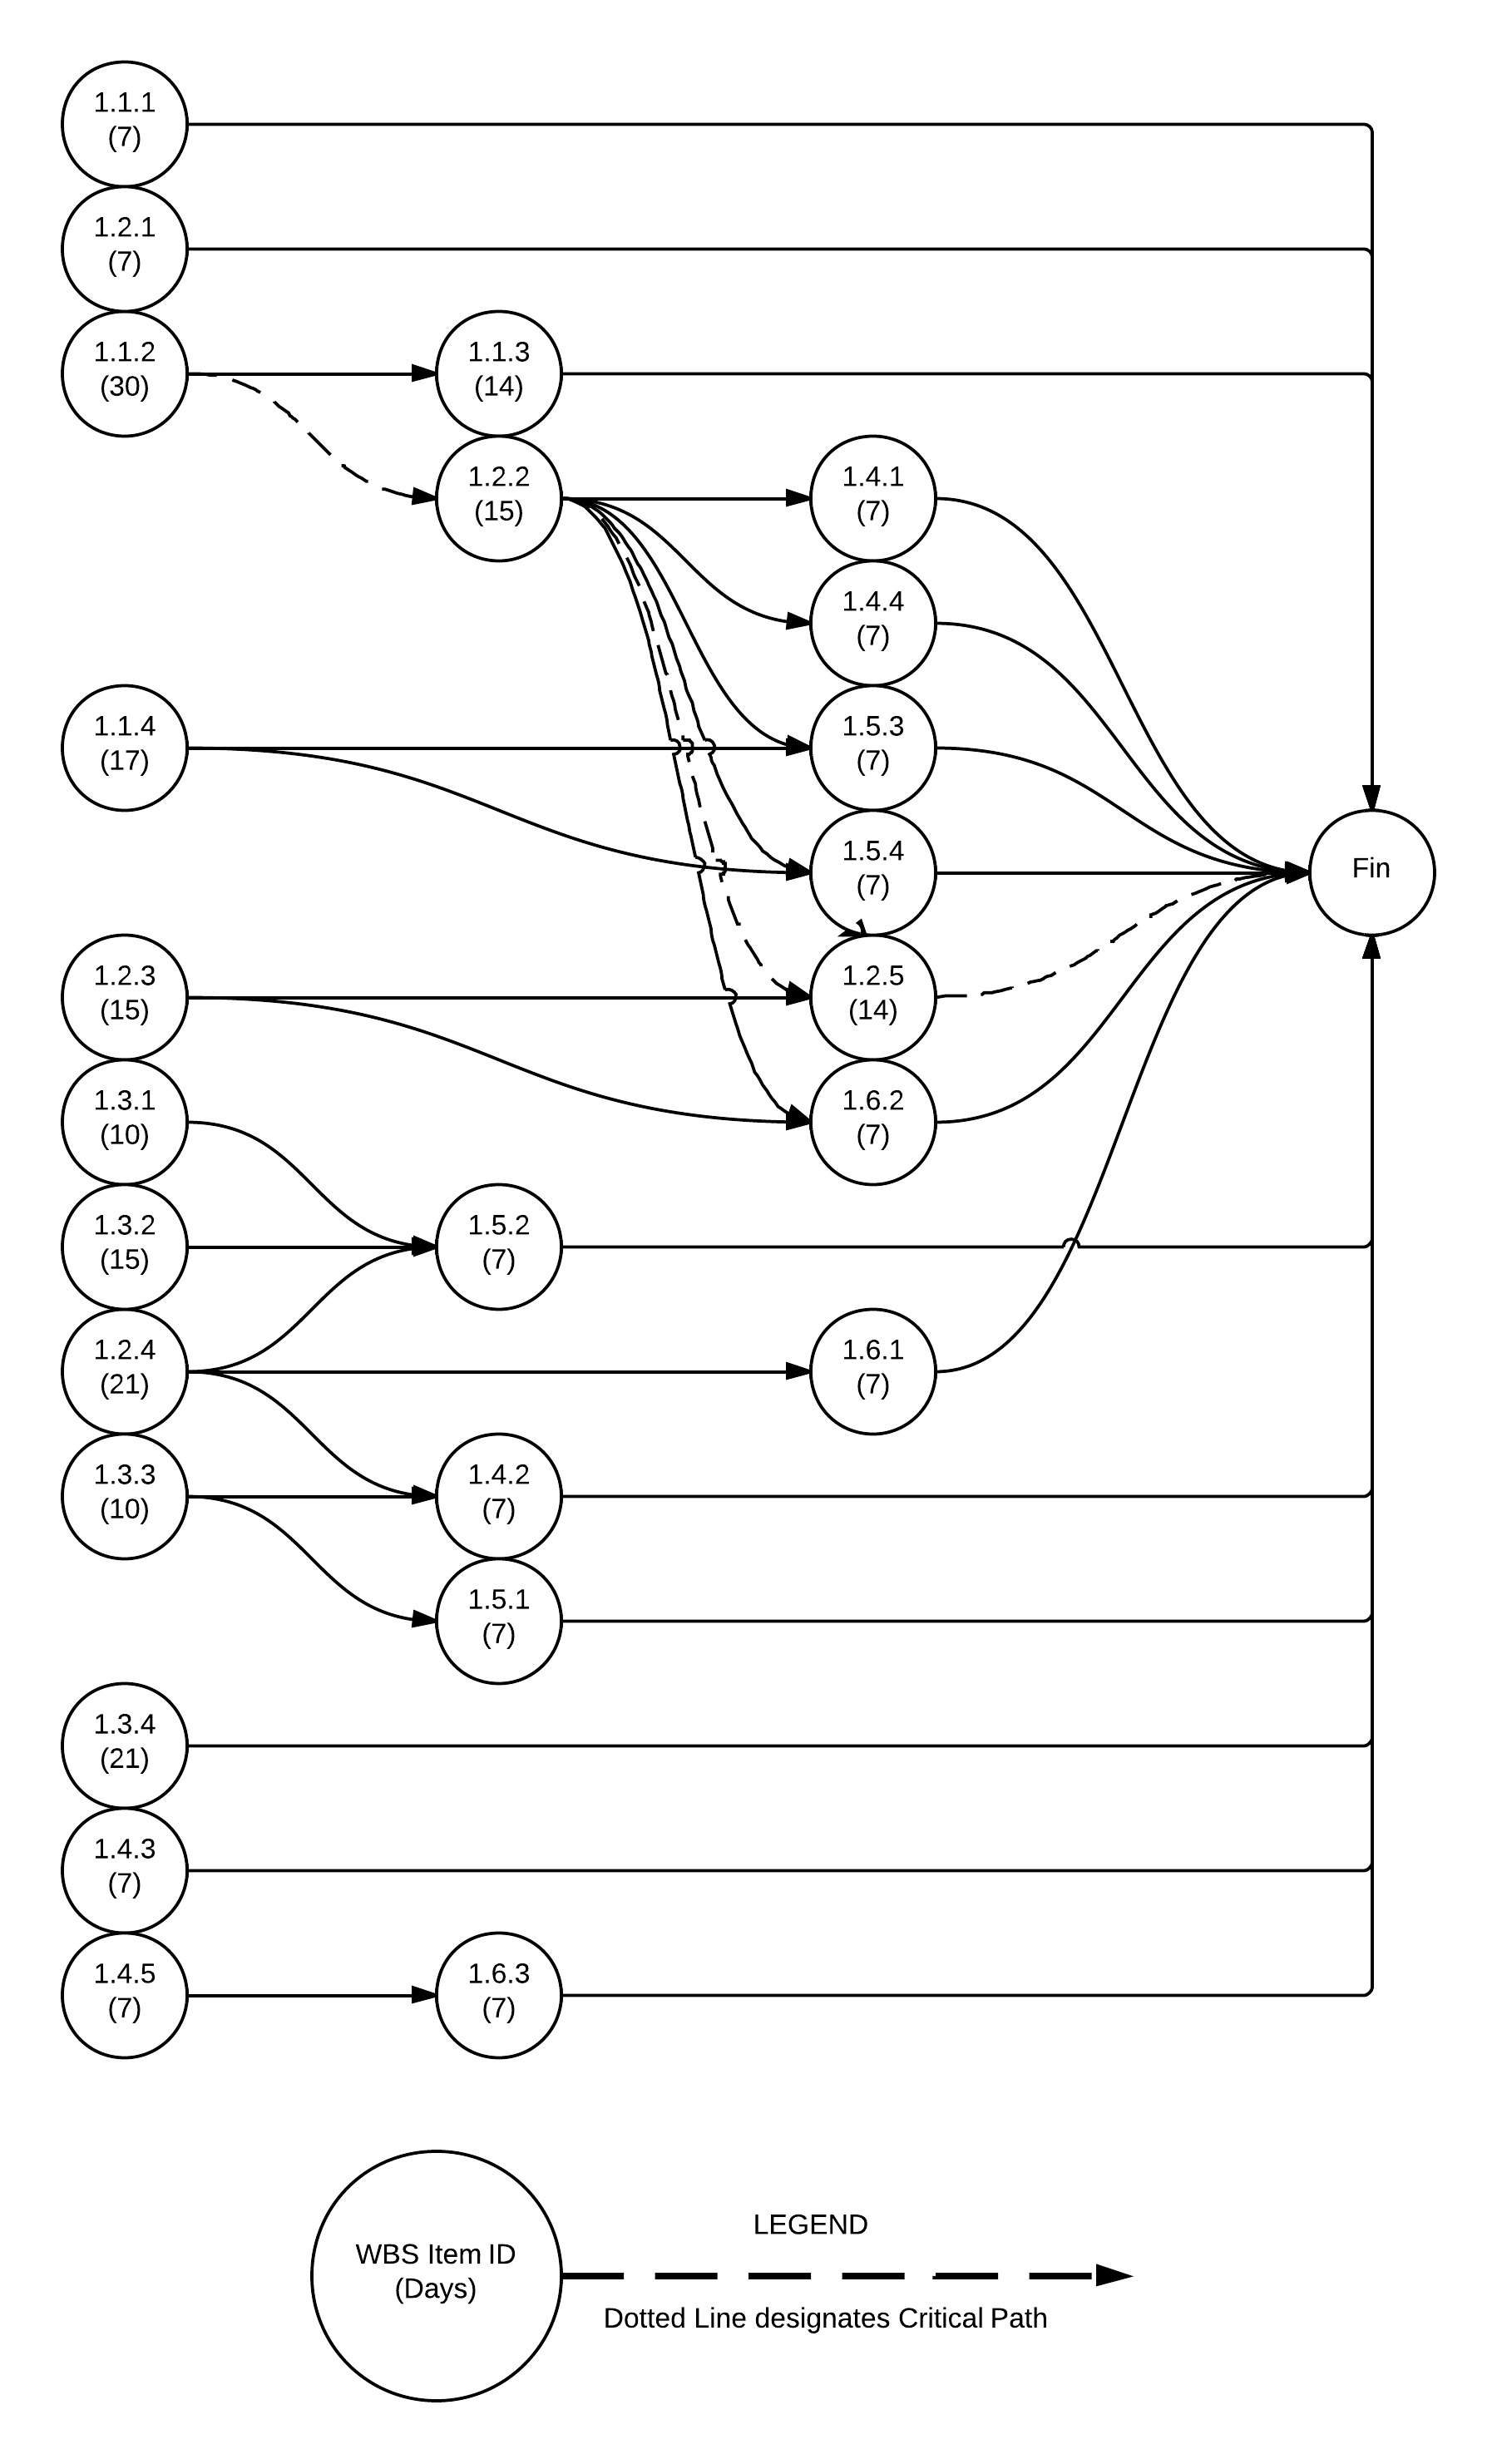
\includegraphics[width=.75\textwidth]{AON.png}
\caption{Activity on Node}
\label{fig:Activity on Node}
\end{figure}
\section{Gantt Chart Schedule}
\begin{figure}[H]
\centering
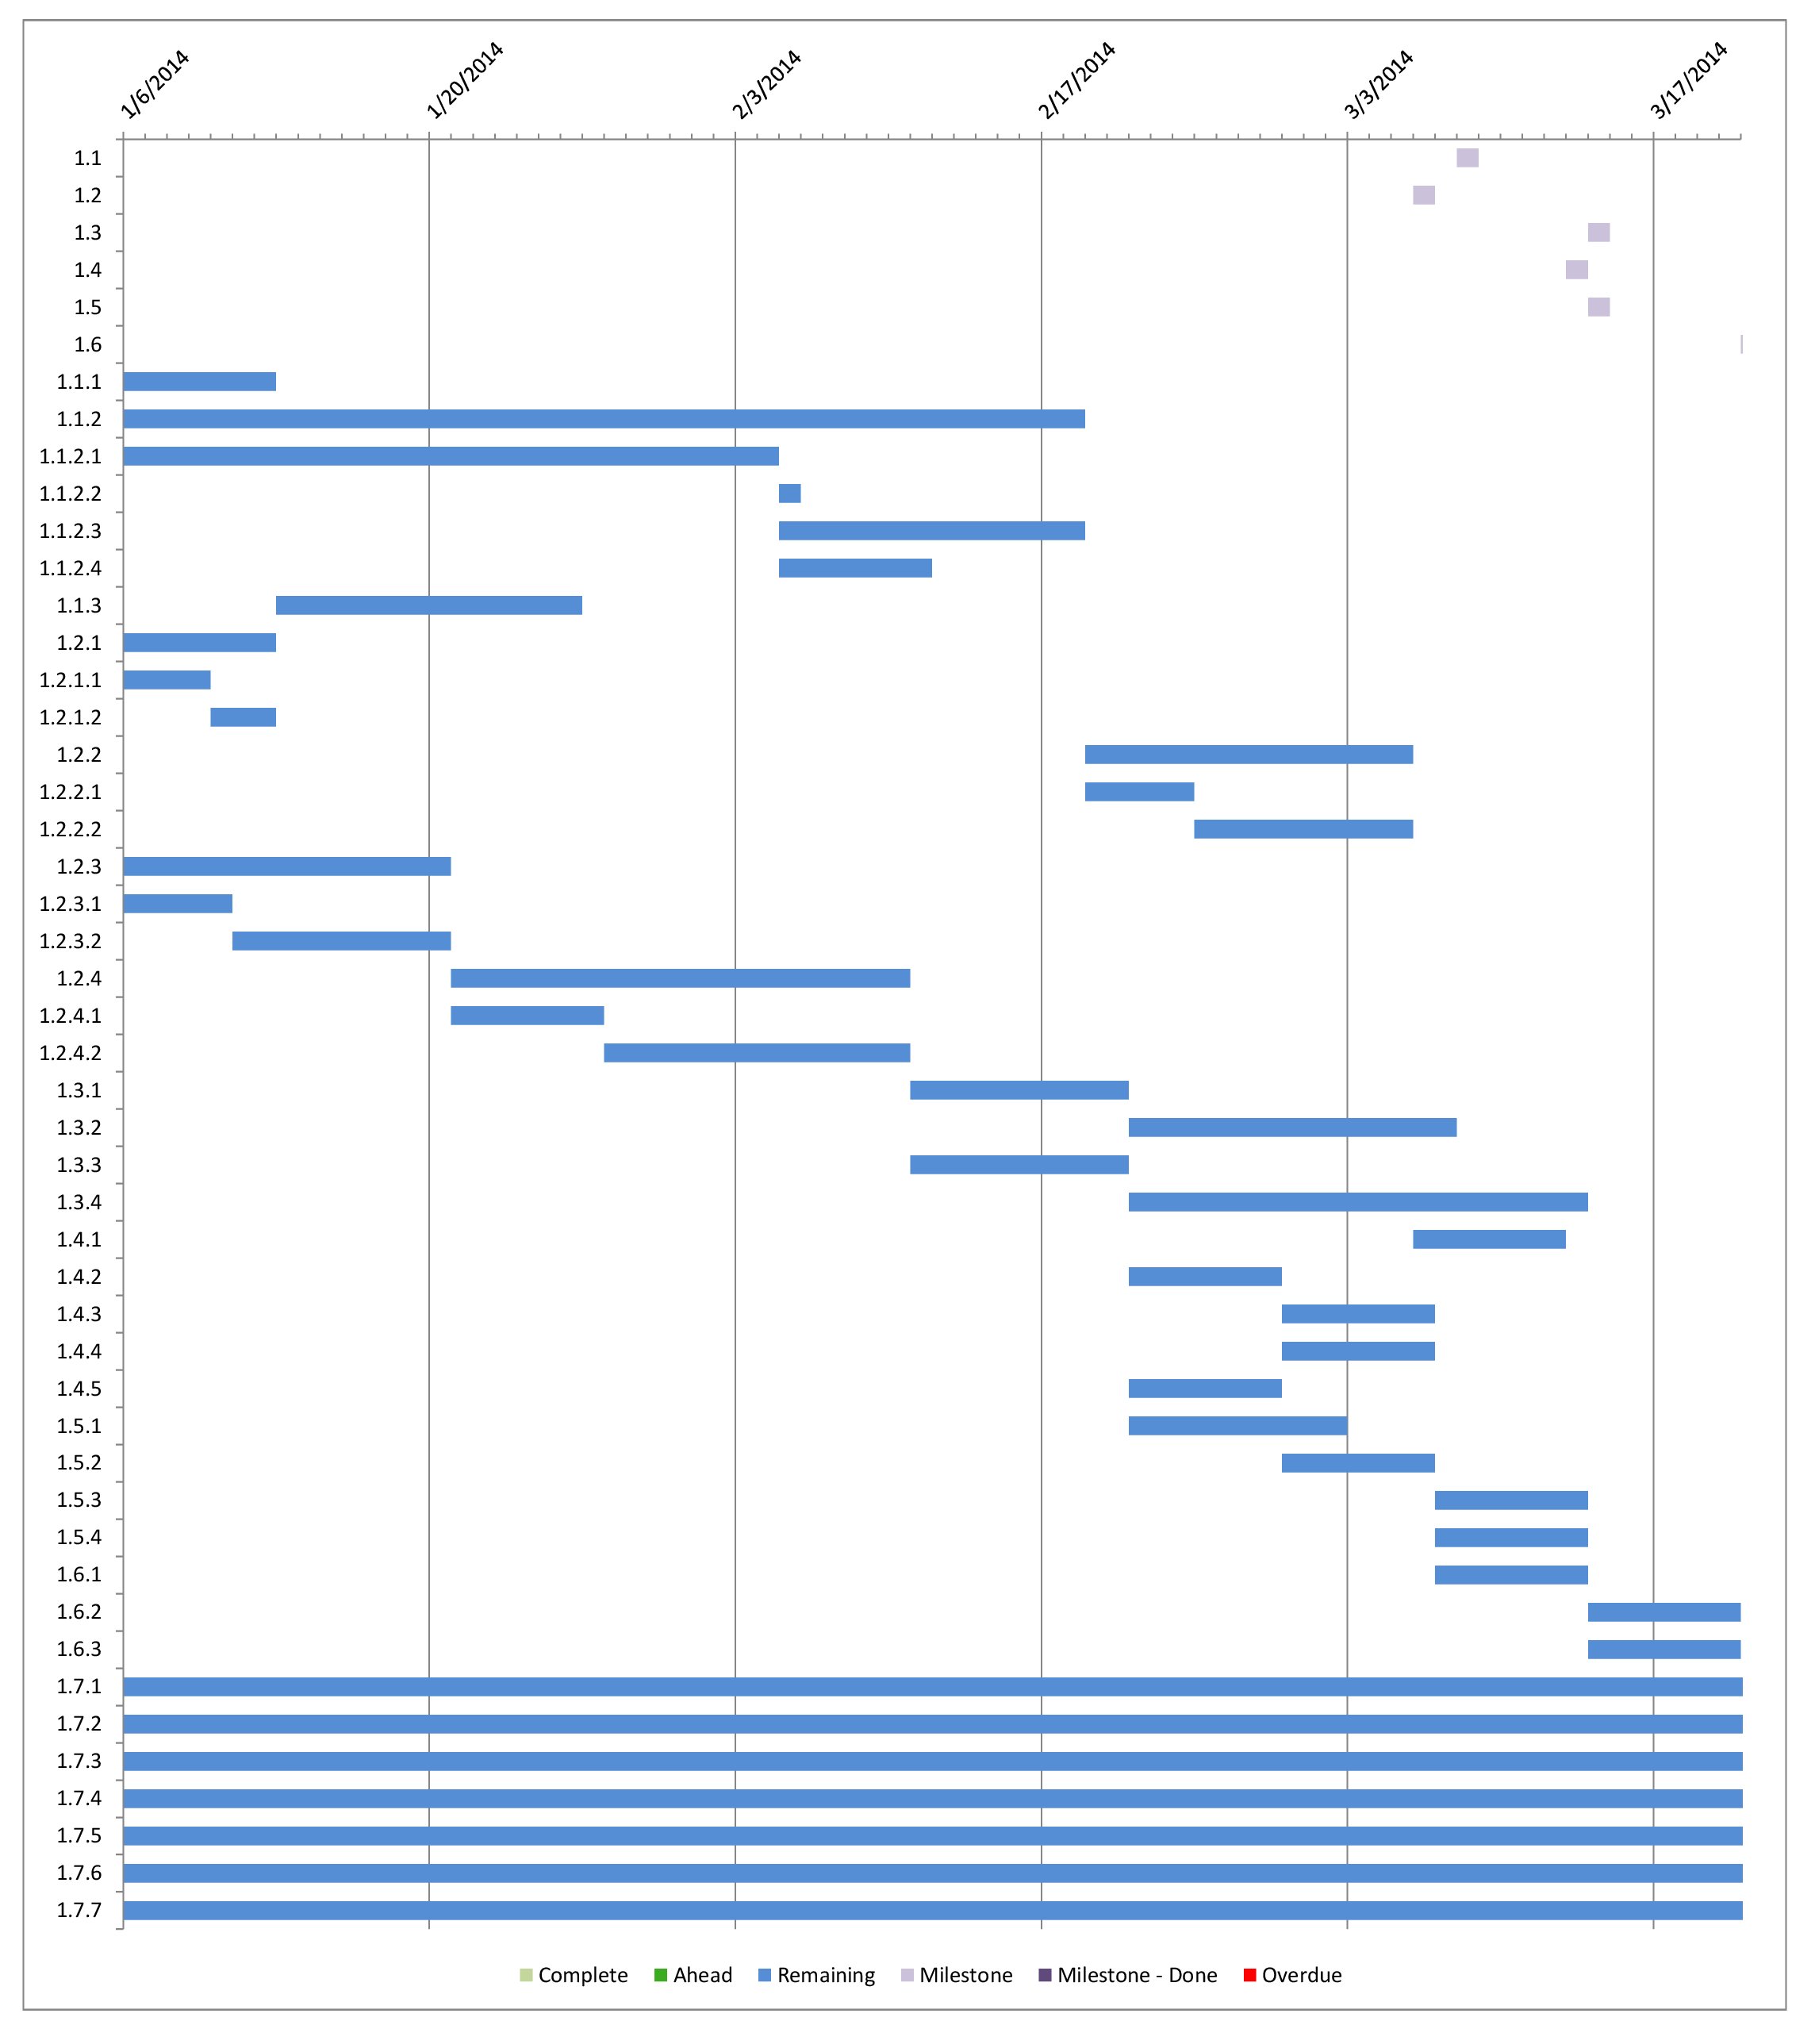
\includegraphics[width=1\textwidth]{gantt.png}
\caption{Gantt Chart}
\label{fig:Gantt Chart}
\end{figure}
\subsection{Landmark Schedule}
Each landmark is marked on the Gantt Chart with a purple square.
\subsection{Critical Design Review Schedule}
Critical design reviews will happen every two weeks, marked on the Gantt Chart by the vertical lines.
Critical design review will end after 6 weeks. By this point the critical parts of the project will be finalized. 
\subsection{Work Breakdown Structure and Linear Responsibility Chart Review and Update Schedule}
Chart updates will happen every two weeks, denoted by both the solid and dashed vertical red lines.
\section{Budget}
\begin{longtable}{|>{\centering}m{3.0cm}|>{\centering}m{1.8cm}|>{\centering}m{1.8cm}|>{\centering}m{1.8cm}|>{\centering}m{1.8cm}|>{\centering}m{2.3cm}|m{1.8cm}|}
	\caption{Budget}
	\label{table:primary} \\
	\hline \textbf{Item} & \textbf{Required} & \textbf{Purchase} & \textbf{Cost} & \textbf{Total} & \textbf{Specification} &\textbf{Supplier}\\ \hline
	\endfirsthead
	\multicolumn{7}{c}{\tablename\ \thetable\ -- \textit{Continued from previous page}} \\ \hline
	 \textbf{Item} & \textbf{Required} & \textbf{Purchase} & \textbf{Cost} & \textbf{Total} & \textbf{Specification} &\textbf{Supplier}
	\endhead 
	\multicolumn{7}{r}{\textit{Continued on next page}} \\
	\endfoot \hline
	\endlastfoot

	Motor Driver Unit&4 &5& \$14.95& \$74.75&DRV 8825&Pololu\\ \hline
	Motor Controller Development Board&1&2&\$35.00&\$70.00& RasPi 512MB&Newark\\ \hline
	Master Controller Development Board&1&2&\$35.00&\$70.00&MSP430 FR5739 Dev Kit&TI\\ \hline
	Peripheral Components&1&2&\$30.00&\$60.00&Misc on-board electronics&Tayda\\ \hline
	Motor Connection Hardware&4&5&\$10.00&\$50.00&8 Pin Mil-Spec Connectors&eBay\\ \hline
	Power Supply Unit&1&2&\$25.00&\$50.00&10A, Switching PSU&eBay\\ \hline
	Testing Materials&1&1&\$50.00&\$50.00&Stuff to carve up&Lowes\\ \hline
	Enclosure&1&1&\$50.00&\$50.00&Fabricate in house&Lowes\\ \hline
	Monitor for\\Master Controller&1&1&\$35.00&\$35.00&HDMI compatible (used)&GoodBytes\\ \hline
	Cabling \& Test Harness&1&2&\$10.00&\$20.00&Wire is expensive&eBay\\ \hline
	Voltage Regulation&2&3&\$6.00&\$18.00&DC-DC Converter&eBay\\ \hline
	Total &&&&\$547.75&&\\ \hline
\end{longtable}
\section{Engineering Hours}

\begin{table}[H] 
\caption{Engineering Hours}
	\label{table:engineeringhours}
	\centering 
\begin{tabular}{|r|c|}
	
	\hline Josh DeWitt&150\\ \hline
	James Gehringer&150\\ \hline
	Evan Milton&150\\ \hline
	Chad Staley&150\\ \hline
	Total&600\\ \hline
\end{tabular}
\end{table} 

\newcommand{\testheader}{\textrotate{\textbf{Step}} & \textbf{Action} & \textbf{Expected Result} & \textrotate{\textbf{Pass}} & \textrotate{\textbf{Fail}} & \textrotate{\textbf{N/A}} & \textbf{Comments} \\ \hline}
\newcommand{\testinfo}[2]{\multicolumn{2}{|r|}{\textbf{Test Case Name:}} & \multicolumn{5}{m{11cm}|}{#1} \\ \hline \multicolumn{2}{|r|}{\textbf{Description:}} & \multicolumn{5}{m{11cm}|}{#2} \\ \hline}
\newcommand{\testerinfo}{\multicolumn{2}{|r|}{\textbf{Name of Tester:}} & & \multicolumn{3}{l|}{\textbf{Date:}} & \\ \hline \multicolumn{2}{|r|}{\textbf{HW/SW Version:}} & & \multicolumn{3}{l|}{\textbf{Time:}} & \\ \hline}
\newcommand{\testsetup}[1]{\multicolumn{2}{|r|}{\textbf{Setup:}} & \multicolumn{5}{m{11cm}|}{#1} \\ \hline}
\newcommand{\testtabular}[3]{\begin{tabular}{|m{.25cm}|m{4cm}|m{5cm}|m{.25cm}|m{.25cm}|m{.25cm}|m{3cm}|}\hline\testinfo{#1}{#2}\testerinfo\testsetup{#3}\testheader}

\chapter{Testing Plan}
Validation and verification prove to all stakeholders that the goals of the project have been met.
Thorough testing throughout the entire project is vital to identifying potential issues and correcting them before a final product is created. 
Validation was completed by comparing the engineering requirements with the marketing requirements that were discussed by the team. 

\section{Verification Metrics}
The following tests will give proof that all of the ten engineering requirements have been met.
\begin{enumerate}
	\item Print out the schematic and the \gls{bom}.
Work through all components on the schematic, placing a check mark next to each component and the corresponding part on the \gls{bom}.
Once the schematic has been fully reviewed, ensure that all items on the \gls{bom} have exactly one check mark next to them.
	\item Use schematic as the netlist for the \gls{pcb} and do not make any manual modifications to the netlist.
Print out the schematic and review it with Professor Detloff to ensure readability.
Verify loading and interface timing analyses through experimental measures using an oscilloscope. 
	\item Generate a \gls{pcb} layout that passes all \gls{drc} operations performed by the \gls{drc} check available at http://www.4pcb.com. 
	\item Use a \gls{dmm} to verify connectivity on all solder joints.
	\item Demonstrate a fully-functional project at the annual senior design showcase. 
\end{enumerate}
\section{Project Milestone Verification}
Landmark milestones will be complete once their associated tests pass.
Table ~\ref{table:testvsland} shows the tests required to be completed for each landmark.

\begin{table}[H]
	\caption{Landmark vs. Required Tests}
	\label{table:testvsland}
	\centering
	\begin{tabular}{|r |c|} 
		\hline\hline
		\textbf{Landmark} & \textbf{Required Tests}\\
		\hline
		\textbf{1.1: Electrical Components} & Step Accuracy, Voltage Supply  \\
		\hline
		\textbf{1.2: Control Software} & G-code Processing  \\
		\hline
		\textbf{1.3: Interface Software} & G-code Processing, Website Test \\
		\hline
		\textbf{1.4: System Testing} & Step Accuracy, G-code Processing, Voltage Supply,\\ 
		& Applications Test, Thermal Shutdown\\
		& Website Test, Serial Link Test \\
		\hline
		\textbf{1.5: Integration Testing} & Automated Regression Testing\\
		\hline
		\textbf{1.6: Unit Testing} & Step Accuracy, G-code Processing, Voltage Supply\\
		\hline 
	\end{tabular}
\end{table}
Test specifications are shown in the Integration, Interface, and Subsystem Testing sections. 
Automated regression testing is run on the \gls{pi} through make, the automated C building tool that processes makefiles.
Regression tests will be written before the code that it is testing.

\subsection{Integration Testing}
\testtabular{Applications Test}{Tests that the system drives 4 stepper motors, 1 DC motor, and 16 GPIO.}{Connect 4 stepper motors and 1 DC motor to motor drivers. Connect test GPIO load to GPIO output. }
	1 & Connect to system through \gls{tcpip}. & System is available and connection is established. & & & & \\ \hline
	2 & Send G-code to system through \gls{tcpip}. & System receives G-code and sends acknowledgment. & & & & \\ \hline
	3 & Send command to execute sent G-code. & System executes the newly received G-code. & & & & \\ \hline
	4 & Verify that all motors respond appropriately. & The 4 stepper motors and 1 DC motor respond appropriately. & & & & \\ \hline
	5 & Verify that all 16 GPIO outputs respond. & The GPIO port responds appropriately. & & & & \\ \hline
\end{tabular}

\testtabular{Thermal Shutdown}{Tests that the system shuts down at CPU temperatures greater than $60^{\circ}C$.}{Prepare the system for normal operation in a test oven.}
	1 & Compare system temperature sensor to ambient temperature. & CPU temperature sensor is within $1^{\circ}C$ of ambient temperature.  & & & & \\ \hline
	2 &  Increase oven temperature to  $55^{\circ}C$. Allow system to run until temperature sensor reaches  $55^{\circ}C$. & System operates normally. & & & & \\ \hline
	3 &  Increase oven temperature to  $62^{\circ}C$. & System shuts off when CPU temperature reaches $60^{\circ}C$.  & & & & \\ \hline
	4 &  Note oven temperature at which system shuts off. & System shuts off before oven temperature exceeds $61^{\circ}C$.  & & & & \\ \hline
\end{tabular}

\subsection{Interface Testing}
\testtabular{Website Test}{Tests that G-code can be uploaded and commands sent through the website over \gls{tcpip} to the \gls{pi}.}{Connect system to network through Ethernet or WiFi. Start up computer that can connect to the same network as the system.}
	1 & Log into Website. & Website comes back with greeting and control panel. & & & & \\ \hline
	2 & Choose a G-code file to upload and press upload. & Website confirms upload was successful. & & & & \\ \hline
	3 & Click to view the uploaded G-code file. & Website shows preview of G-code, which matches the uploaded file. & & & & \\ \hline
\end{tabular}

\testtabular{Serial Link Test}{Tests that the \gls{pi} and the slave device can communicate serially}{Load serial test code onto \gls{pi} and the slave device.}
	1 & Connect the \gls{pi} and the slave device, power on the system, and connect directly with the \gls{pi}. & \gls{pi} and slave device start up with no errors. & & & & \\ \hline
	2 & Start the serial link test program on the \gls{pi}. & \gls{pi} sends data to the slave device and the slave device responds with the correct 8-bit modulo sum. & & & & \\ \hline
\end{tabular}

\subsection{Subsystem Testing}
\testtabular{Stepper Motor Accuracy}{Tests that the stepper motor pulses are accurate.}{Configure oscilloscope to measure the frequency of input 1. Set a constant running frequency of 10kHz on all motors through G-code.}
	1 & Connect oscilloscope to the input of the first stepper motor driver. & Oscilloscope measures within 5\% of 10kHz. & & & & \\ \hline
	2 & Repeat the previous step for the second, third, and forth stepper motor drivers. & Oscilloscope measures within 5\% of 10kHz. & & & & \\ \hline
\end{tabular}

\testtabular{G-code Processing}{Checks that G-code can be successfully processed by the system.}{Directly connect to \gls{pi} through a shell.}
	1 & Run all automated G-code processing tests. & All tests pass and no errors are reported. & & & & \\ \hline
	2 & Create a sample G-code file for creating a square locally on the \gls{pi}. & File is saved in an accessible directory. & & & & \\ \hline
	3 & Run G-code processing on sample G-code file. & System successfully interprets the G-code and outputs a file with instructions to the motor driver to draw a square. & & & & \\ \hline
\end{tabular}

\testtabular{Voltage Supply}{Tests that the system operates between 14-36V.}{Connect system to variable power supply with a range of at least 14-36V or seperate power supplies with voltages of 14V, 25V, and 36V.}
	1 & Set power supply to 14V. & \gls{pi} voltage supply is 5V. Microcontroller voltage supply is 5V. Motor Controller voltage supply is TBD.  & & & & \\ \hline
	2 &  Set power supply to 25V. & \gls{pi} voltage supply is 5V. Microcontroller voltage supply is 5V. Motor Controller voltage supply is TBD. & & & & \\ \hline
	3 & Set power supply to 36V. & \gls{pi} voltage supply is 5V. Microcontroller voltage supply is 5V. Motor Controller voltage supply is TBD. & & & & \\ \hline
\end{tabular}

\begin{appendices}
	\chapter{Project Charter}

\section{Roles and Authority}
The following definitions will serve as the guidelines for each team member's major tasks throughout the project lifetime. 
All team members are expected to help one another out to ensure the best outcomes for the project, not just for the individual's task completion.

\subsection{Faculty Sponsor: Herbert Detloff}
Demonstrates previous experience with several successful Senior Thesis Projects.
Provides feedback and assessment of project definition, plan, and status.
Ensures that all team members are aware of the engineering impact of the project on the University of Nebraska - Lincoln and the rest of the world.
Teaches standard engineering principals for project management, development, execution, and testing to aid in the project's completion.

Reports to the \gls{ceen} Department.

\subsection{Resource Manager: James Gehringer}
Responsible for promoting collaboration, communicating progress with the faculty sponsor, and procuring resources.
Accountable for intellectual property management in solidification of ideas and iterative verification of project objectives.
Involved with all phases of design in order to better assure both long and short term goals are met with efficiency by keeping track of the progress of the project by setting deadlines, scheduling tasks, and monitoring progress through tools such as Gantt charts.
Oversees documentation and monitors project health to identify issues as soon as possible.

Reports to the Faculty Sponsor. 

\subsection{Systems Engineer: Evan Milton}
In charge of generating the system's requirements and specifications and understanding the project as a whole, including mechanical, electronic, and software components and their interfacing.
Works closely with the Hardware and Software Development Engineers to best meet the team objectives, system's requirements, and specifications.
Responsible for acceptance testing the prototypes and final project to ensure quality and confirm that all specifications are met.
Determines alternate solutions case any solution fails or becomes unfeasible during development.
Makes final design decisions when challenges arise that require major modifications.

Reports to the Resource Manager and Faculty Sponsor.

\subsection{Hardware Development Engineer: Chad Staley}
Accountable for developing the design, layout, construction, and testing of the electrical systems required for this project to create a solid platform for the software.
Will focus on simplicity and robustness in design to aid in troubleshooting when software is added to the project.
Understands and can communicate the software interfacing that must occur to make the hardware function properly.

Reports to the Systems Engineer, Resource Manager, and Faculty Sponsor. 

\subsection{Software Development Engineer: Josh Dewitt}
Responsible for the higher level functionality of the project by writing clean, modular code that can be adapted where hardware changes might be cost-prohibitive.
Will communicate with the Hardware Development Engineer to understand the hardware interfacing to meet the requirements set by the Systems Engineer.
Performs domain, software element, and requirements analysis to ensure the code produced matches the needs of the users, then develops code in any language necessary, using test­-driven development.

Reports to the Systems Engineer, Resource Manager, and Faculty Sponsor.

\section{Development Methodology}
The project definition was chosen to use all of the engineers' talent, while still being achievable given the time frame of the course.
The goal of this project is to create a final high-quality system that is reproducible, robust, and goes beyond expectations.
This goal will be achieved through proper planning, developing hardware and software in parallel, applying rapid prototyping and \gls{xp} techniques to hardware and software development, and focusing on system testing throughout the process.
Development methodologies will determine how quickly and accurately the project plan can be executed. 

\subsection{Hardware}
The goal of the hardware development is to create reliable circuits that meet design requirements.
Circuits will be simulated using CircuitLab when possible and prototyped using a breadboard.
Upon passing initial simulation and testing, hardware prototypes will be quickly developed using a \gls{cnc} to mill \gls{pcb}s developed in Eagle \gls{cad}.
The \gls{pcb}s will then be populated, allowing software integration and testing to begin.
Prototypes that pass testing will be sent to a manufacturer to create a final product.
An accurate \gls{bom} will be generated for all final hardware modules.

\subsection{Software}
The goal of the software development is to create reliable programs that can be understood and maintained over the course of the Senior Thesis Project and beyond.
\gls{xp} techniques will be used for software development to allow greater flexibility in the system and allow more rapid feature implementation and ensure that the software components are fully integrated with the hardware components. 
\gls{xp} techniques will save time in the long run, as undocumented, untested, and difficult-to-understand code will take more time for modifications and consume more resources for debugging issues.
The most notable \gls{xp} techniques to be used are unit testing, pair programming, and stand-up meetings.

\paragraph{Unit Testing}
Programming through unit testing simply means that code for runtime is never written until a failing test proves that it is needed, ensuring that all code is written for a reason.
Invalid inputs can be provided to code to test boundary conditions that are difficult to produce in acceptance testing, decreasing the number of bugs in code.
Unit testing also enforces that the inputs, outputs, and use of code are fully documented, while verifying code throughout development. 

Automated unit testing that can easily be run at any time ensures that code is written modularly, provides verification throughout development, and checks that new changes do not break existing features of the code.
Whenever a test fails after making a change, the developer can analyze the test to understand how their change caused the test to fail, ultimately correcting the problem before it is fully implemented in the system.
 
\paragraph{Pair Programming}
One person on a small project team performing all development, creates "knowledge silos" that can halt development if the person leaves the team.
Software limitations may restrict other design choices, including hardware design, so software knowledge will be spread throughout the team, improving the quality of the final product. 

Pair programming helps prevent small bugs from being introduced into the code, which can save time throughout software development.
Software bugs are most easily found and corrected shortly after being written, as the engineer is still familiar with that code, so the extra hours can quickly pay off.

\paragraph{Stand-up Meetings}
The most important implication of stand-up meetings is the ability to keep software development on time.
The meeting is performed while standing, to ensure brevity and allow all parties to get back to work as soon as possible.
Despite not taking long, simply discussing the current stage in the development process allows individuals to express any potential roadblocks that may exist and discuss issues they are having.
Another individual on the team will often have useful input and may help avoid roadblocks and solve errors, ultimately keeping development on schedule. 

\section{Project Control}
The project will focus on the punctual production of functional deliverables at set deadlines, tracked in a Gantt chart.
The Resource Manager will be able to concretely monitor project status, and inform members of changes in course as they become necessary.
Detailed documentation of all efforts will be maintained in each person's engineering logbook.

\subsection{Communication Channel}
Face-to-face group status meetings in PKI 330G will be held to update the status of each deliverable being worked on and provide proactive feedback to keep the project on track.
As much communication as possible will be done in person, as opposed to through phone, text, or email conversations because of the higher information bandwidth.
A wiki for the project, hosted on wikispaces.com, will be used to maintain documentation that will be useful during development and for the final users. 
The website kanbanpad.com, an online project tracking tool, will be used to update the status of tasks between the planning, designing, development, testing, and release phases of project development.
Room PKI 330G will be used for any additional meetings required, which may or may not include the entire team.

\subsection{Communication Frequency}
The face-to-face status meetings will be held twice a week to keep each member aware of the overall progress.
All team members are encouraged to use PKI 330G as the primary work area for the project to increase collaboration and encourage spontaneous discussion regarding the project.
All team members will update the status of their tasks on kanbanpad.com as soon as they change between one of the stages, allowing all members to see the most up-do-date project status wherever they are.

\begin{minipage}{\textwidth}
\section{Team Member Sign-off}
By signing below, I agree to the project charter and acknowledge my required contributions to the Senior Thesis Project.
I understand that failure to adhere by the rules set forth in this project charter will result in negative consequences as deemed fit by the remaining team members and the Faculty Sponsor. 

\signatures
\end{minipage}

	\chapter{Team Meeting Minutes}
\minutesessentials{19}{2013-12-03}{15:00-15:25}{PKI 201C}{Present}{Present}{Present}{Present}
\minutesdetails
{
	\item Receive feedback from Detloff on the Project Plan.
	\item Determine which modifications to the report will be required.
	\item Review the \gls{pssc} with Detloff to improve upon the engineering requirements.
	\item Schedule time to meet for questions regarding the project proposal.}
{
	\item The critical path will be marked on the \gls{aon}.
	\item The milestones will be explained better for easier understanding. 
	\item etc. etc. etc.
}

\signatures
\end{appendices}
\end{document}
